%\documentclass[spanish,12pt,a4paper,titlepage,twoside,openright]{scrbook}
\documentclass[12pt,a4paper,titlepage]{report}
%\usepackage[latin1]{inputenc}
\usepackage[utf8]{inputenc}
\usepackage{graphicx}
\usepackage{subfig}
\usepackage{float}
\usepackage{wrapfig}
\usepackage{multirow}
\usepackage{caption}
\usepackage[spanish]{babel}
\usepackage[dvips]{hyperref}
\usepackage{amssymb}
\usepackage{listings}
\usepackage{epsfig}
\usepackage{amsmath}
\usepackage{array}
\usepackage[table]{xcolor}
\usepackage{multirow}
\usepackage{hhline}
\usepackage{cancel}

\usepackage[Sonny]{fncychap}
%\usepackage[Glenn]{fncychap}
%\usepackage[Conny]{fncychap}
%\usepackage[Rejne]{fncychap}
%\usepackage[Bjarne]{fncychap}

\usepackage{subfiles}
\usepackage{framed}
\usepackage{appendix}
\setlength{\topmargin}{-1.5cm}
\setlength{\textheight}{25cm}
\setlength{\oddsidemargin}{0.3cm} 
\setlength{\textwidth}{15cm}
\setlength{\columnsep}{0cm}
%\setkomafont{disposition}{\normalfont\bfseries}
\captionsetup{tablename=Tabla}

\ChNameVar{\bfseries\LARGE\sf}\ChNumVar{\fontsize{62}{65}\selectfont}
\ChTitleVar{\bfseries\LARGE\sf} \ChRuleWidth{2pt} \ChNameAsIs
\ChTitleAsIs
\renewcommand\FmN[4]{}
\newcommand{\HRule}{\rule{\linewidth}{0.5mm}}

\begin{document}


\begin{titlepage}
\begin{center}
\vfill
%\vspace{50cm}
\textsc{\LARGE Facultad de Ingenier\'ia de la Universidad de la Rep\'ublica}\\[1.5cm]
\vspace{2cm}
\textsc{\LARGE Procesamiento Digital de Señales de Audio\\[1cm]Curso 2012}\\[0.5cm]
\vspace{2.3cm}
% Title
\HRule \\[0.4cm]
{ \huge \bfseries Beat Tracking}\\[0.4cm]
\HRule \\[1.5cm]
\vspace{2cm}
% Author and supervisor
%\begin{center}
\begin{minipage}{0.4\textwidth}
\begin{flushleft} \large
\emph{Autores:}\\
%\begin{center}
%\begin{LARGE}
Gonzalo \textsc{Gutiérrez}\\ Mat\'ias \textsc{Tailani\'an}
%\end{LARGE}
%\end{center}
\end{flushleft}
\end{minipage}
%\end{center}
\begin{minipage}{0.4\textwidth}
\begin{flushright} \large
\end{flushright}
\end{minipage}

\vspace{2cm}

\vfill
\begin{figure} [h!]
\centering
\subfloat{
\includegraphics[width=0.25\textwidth]{./pics/logoIIE_transparente.png}}\hspace{1cm}
\subfloat{
\includegraphics[width=0.15\textwidth]{./pics/logo_fing_transparente.png}}\hspace{1cm}
\subfloat{
\includegraphics[width=0.15\textwidth]{./pics/logo_udelar.png}}
\end{figure}

% Bottom of the page
{\large \today}
\end{center}
\end{titlepage}



\chapter*{Introducción}

Al escuchar música una reacción inconsciente muy común es mover el pie golpeando el piso a tiempo con el \textbf{beat}. La tarea computacional que intenta replicar ese comportamiento es conocida como \textbf{beat tracking}.\\

La métrica de la señal se puede pensar como una estructura de pulsos percibidos a diferentes escalas temporales en una pieza musical. Se consideran 3 niveles métricos básicos: el \emph{tatum}, el \emph{tactus} o \emph{beat} y el \emph{compás}. El tatum es el valor en tiempo más pequeño que puede encontrarse en una pieza musical, es la unidad atómica de la pieza. En general los otros valores de duración presentes en la pieza son múltiplos de tatum. El tactus o beat está más relacionado con el aspecto semántico, y está directamente vinculado con el \textbf{tempo} de la pieza. Por último el compás está vinculado con la tasa de cambios armónicos o la duración de un patrón rítmico.\\

El problema del seguimiento de beat o \emph{beat tracking} es un problema todavía abierto, donde se sigue intentando con gran actividad lograr mejorar los resultados del estado del arte. Tiene un atractivo muy importante en sí mismo pensando en aplicaciones como el acompañamiento automático, asistencia a la hora del editado, estudios musicológicos, efectos de música adaptativos, o seguimiento del ritmo de una batería tocando en vivo, pero además es una parte imprescindible de algunos sistemas más complejos para aplicaciones como etiquetado de música, reconocimiento automático del género, análisis de similitud de música y para lograr la \emph{transcripción automática de música}.\\

El presente trabajo presenta un algoritmo de seguimiento de \emph{beat} de una pieza musical y se basa en el trabajo de ``Jo\~ao Lobato Oliveira, Fabien Gouyon, Luis Gustavo Martins, Luis Paulo Reis'', titulado ``IBT: A real time tempo and beat tracking system, presentado en la \emph{$11^a$ International Society for Music Information Retrieval Conference, ISMIR}, en 2010'' (\cite{bib:el_posta}). Dicho trabaja se basa a su vez en el sistema \textbf{BeatRoot}, presentado en (\cite{bib:dixon}): Dixon S., ``Automatic extraction of tempo and beat from expressive performances.'', \emph{Journal of New Music Research}, 2001. De \cite{bib:dixon} se toma la idea de varios \textbf{agentes} compitiendo y llevando varias hipótesis de tempo y fase paralelamente, se agrega robustez ante entradas ruidosas y se implementa en tiempo real. Aún realizando todas las operaciones de forma causal y en tiempo real, se logra obtener resultados comparables con el estado del arte y se convierte además en el primer software \emph{open source} de seguimiento de beat en tiempo real.


\chapter{Metodología}
\label{sec:metodologia}

Como se puede ver en la figura \ref{fig:bloques} el algoritmo consta de 3 fases fundamentales:
\begin{itemize}
\item \textbf{Audio Feature Extraction}: En esta etapa se trasforma la señal de audio en 1 secuencia contínua que caracteriza la información más relevante para el análisis rítmico. En esta etapa se basarán las siguientes partes del algoritmo.
\item \textbf{Pre-Tracking}: Al finalizar el Pre-Tracking se tendrá un conjunto de hipótesis iniciales con respecto a posibles períodos y fases de los beats. Consta de 3 subetapas donde se estimarán las características que definen a un agente:
\begin{itemize}
\item Período
\item Fase
\item Puntaje
\end{itemize}
\item \textbf{Beat-tracking}: En esta etapa se propagan las hipótesis y se crean, matan y puntúan agentes.
\end{itemize}

A su vez se presenta un sistema de evaluación que decide en función del puntaje de cada agente, cúal es el más adecuado para la pieza musical: el \textbf{Agent Referee}.

\begin{figure}[h!]
\centering
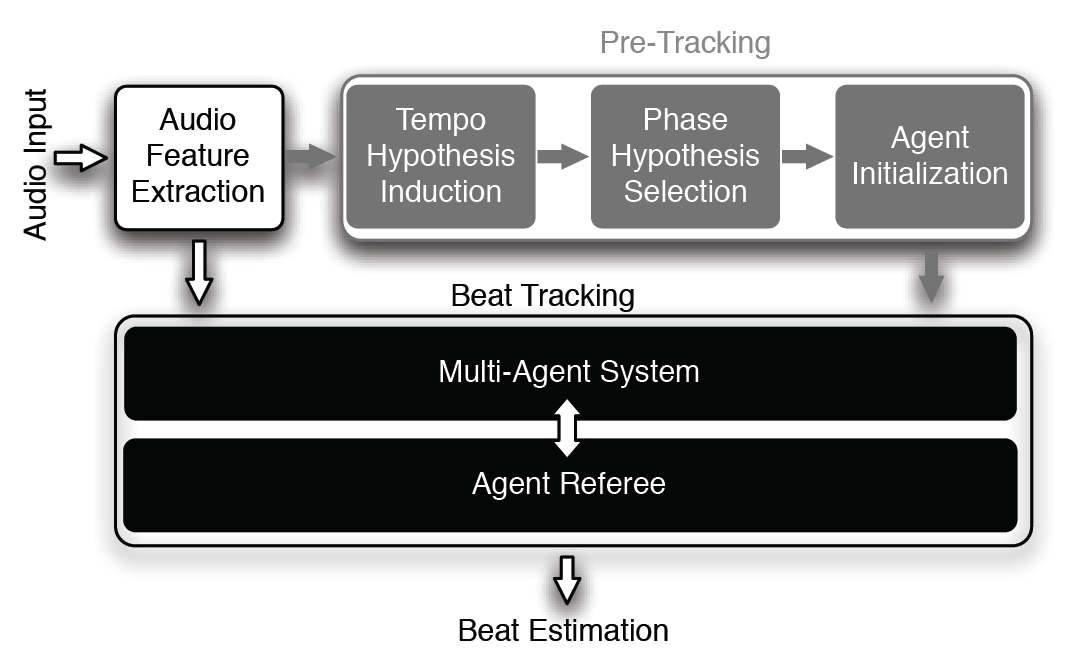
\includegraphics[width=.6\linewidth]{./pics/bloques}
\caption{Diagrama de bloques}
\label{fig:bloques}
\end{figure}

\section{Audio Feature Extraction}
En \cite{bib:feature_extraction} se evalúan distintas magnitudes para caracterizar la información más relevante para el análisis rítmico. Está fuera del alcance del presente trabajo analizar la posibilidad de evaluar distintas magnitudes, por lo que se trabajará con el \textbf{Flujo Espectral} como magnitud característica de la pieza musical.\\

El flujo espectral utiliza una representación tiempo-frecuencia de la señal basada en la trasformada corta de Fourier utilizando una ventana de Hamming, $w(m)$.\\

$X(n,k)$ representa al k-ésimo bin de frecuencia del n-ésimo frame, como se ve en la ecuación \ref{ec:x}
\begin{eqnarray}
X(n,k)=\sum\limits_{m=-\frac{N}{2}}^{\frac{N}{2}-1} x(hn+m)w(m)e^{-\frac{2\pi jmk}{N}}
\label{ec:x}
\end{eqnarray}

El flujo espectral lleva una medida del cambio en magnitud de cada \emph{bin} de frecuencia restringido a cambios positivos y sumado a lo largo de todos los \emph{bins} de frecuencia. En la ecuación \ref{ec:sf} se muestra su ecuación matemática para el cálculo.
\begin{eqnarray}
SF(n)=\sum\limits_{k=-\frac{N}{2}}^{\frac{N}{2}-1} H(|X(n,k)|-X(n-1,k)|)
\label{ec:sf}
\end{eqnarray}
donde $N=2048$ (46 $ms$ a una frecuencia de muestreo $r=44100Hz$) y el tamaño del salto es $h=441$ (10 $ms$ o 78\% de solapado). $H(x)$ es un rectificador de media onda: $H(x)=\frac{x+|x|}{2}$.


%TODO figura

\section{Pre-Tracking}
\label{sec:pretracking}

La etapa del Pre-Tracking es fundamental ya que en ella se basarán las etapas siguientes del algoritmo. Se analiza una \emph{ventana de inducción} de 5 segundos y se obtiene como salida un conjunto de agentes caracterizados por $(P_i,\phi _i, S_i) $ para cada agente $i=1\dots N$. Consta de 3 sub-etapas donde se calcula el período ($P_i$), fase ($\phi _i$) y puntaje ($S_i$) de cada agente $i$.

\subsection{Período}
La primera etapa consiste en hallar una función de periodicidad continua basada en la autocorrelación y el Flujo Espectral:
\begin{equation}
	A(\tau) = \sum\limits_{n=0}^{m}SF(n)SF(n+\tau)
	\label{ec:autocorrelacion}
\end{equation}
La segunda etapa consiste en la detección de eventos, por medio de un hallado y filtrado de picos de la función de autocorrelación descripta anteriormente (ecuación \ref{ec:autocorrelacion}). Los eventos detectados en $A(\tau)$ corresponderán con los períodos iniciales de los agentes del Pre-Tracking. El criterio propuesto para obtener dichos picos es:
\begin{equation*}
	\begin{cases}
	P_i = \arg\max_i \left\{ A(\tau) \right\}, & i=1,\dots, N\\
	A(\tau)>\delta \frac{rms(A(\tau))}{M} & 
	\end{cases}
	\label{ec:period}
\end{equation*}
$\delta$ es un umbral determinado empíricamente en $0.75$ y $M$ es un rango de tiempos definido entre [50,250] BPM.

%TODO figura y explicar que es lo q agregamos nosotros

\subsection{Fase}

Para cada $P_i$ estimado se generan $j$ hipótesis para la fase: $\phi_i^j$. Se supone fase y períodos constantes en cada ventana de análisis.\\

Se utiliza un \emph{template} de tren de pulsos isócronos para ver cuál ajusta mejor a los picos del Flujo Espectral en la ventana de inducción.\\

Utilizando un proceso de tracking simplificado como veremos en la sección \ref{sec:tracking} se selecciona el tren de pulsos que mejor ajusta los eventos detectados. Hasta este momento tenemos una pareja $(P_i,\phi _i)$ para cada agente.

\subsection{Puntaje}

A cada pareja $(P_i,\phi _i)$ se le asigna un puntaje preliminar $S_i^{raw}$ que corresponde a la suma de los errores entre los elementos del tren de pulsos y los máximos locales del Flujo Espectral, dado por la ecuación \ref{ec:ds}.\\

\begin{wrapfigure}{l}{0.45\textwidth}
	\vspace{-25pt}
	\begin{center}
	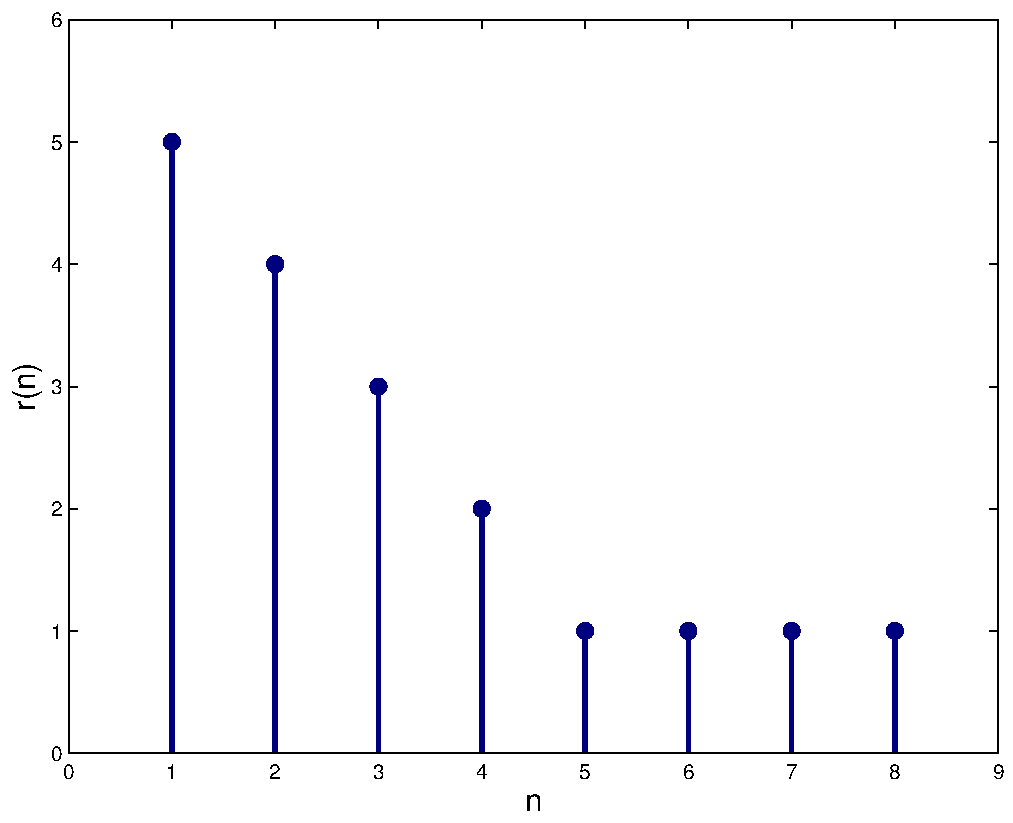
\includegraphics[width=0.4\textwidth]{./pics/r.pdf}
	\end{center}
	\vspace{-20pt}
	\caption{r(n)}
	\label{fig:r}
	\vspace{-35pt}
\end{wrapfigure}

Luego considerando relaciones métricas entre pares de hipótesis de período ($n_{ij}$), se actualiza el puntaje a:
$$S^{rel}_i=10S_i^{raw}+\mathop{\sum\limits_{j=0}^{N}}_{j \neq i}r(n_{ij})S_j^{raw}$$ donde 
$$r(n)= \begin{cases}
6-n, & 1\leq n \leq 4\\
1, & 5\leq n \leq 8\\
0, & en\;otro\;caso
\end{cases}
$$

que también se puede ver representada en la figura \ref{fig:r}. El resultado de aplicar la función $r(n)$ es favorecer todos los agentes que tengan múltiplos enteros uno de otro.\\

Por último el puntaje final está dado por:
\begin{equation}
S_i=\frac{S_i^{rel}}{\max S_i^{rel}}\max S_i^{raw}
\label{ec:S}
\end{equation}

Tenemos entonces un conjunto de agentes, donde cada uno de ellos está caracterizado por una tríada $(P_i,\phi _i,S_i)$ que serán utilizados como hipótesis iniciales para la etapa de \textbf{Tracking}.

\section{Beat-Tracking}
\label{sec:tracking}

La idea de la etapa de Tracking es supervisar flujo de entrada de los picos detectados del Flujo Espectral y mantener un buen balance entre inercia y rapidez de la respuesta ante cambios.\\

Cada predicción es evaluada respecto de su desviación al máximo local correspondiente en los datos observados, considerando una ventana como se la mostrada en la figura \ref{fig:grafica}, donde se consideran 2 intervalos de tolerancia:
\begin{itemize}
\item \emph{inner}: $T_{in}\in[T_{in}^l,T_{in}^r]$ con $T_{in}^l=T_{in}^r=46.4ms$ para manejar pequeñas desviaciones de fase y período
\item \emph{outer}: $T_{out}\in[T_{out}^l,T_{in}^l] \bigcup [T_{in}^r,T_{out}^r]$ con $T_{out}^l=0.2\;P_i$ y $T_{out}^r=0.4\;P_i$ para contemplar eventuales cambios repentinos de tiempo. La asimetría refleja una mayor tendencia a disminuir el tempo.\\
\end{itemize}

\begin{figure}[h!]
  \begin{center}
  \vspace*{-10pt}
  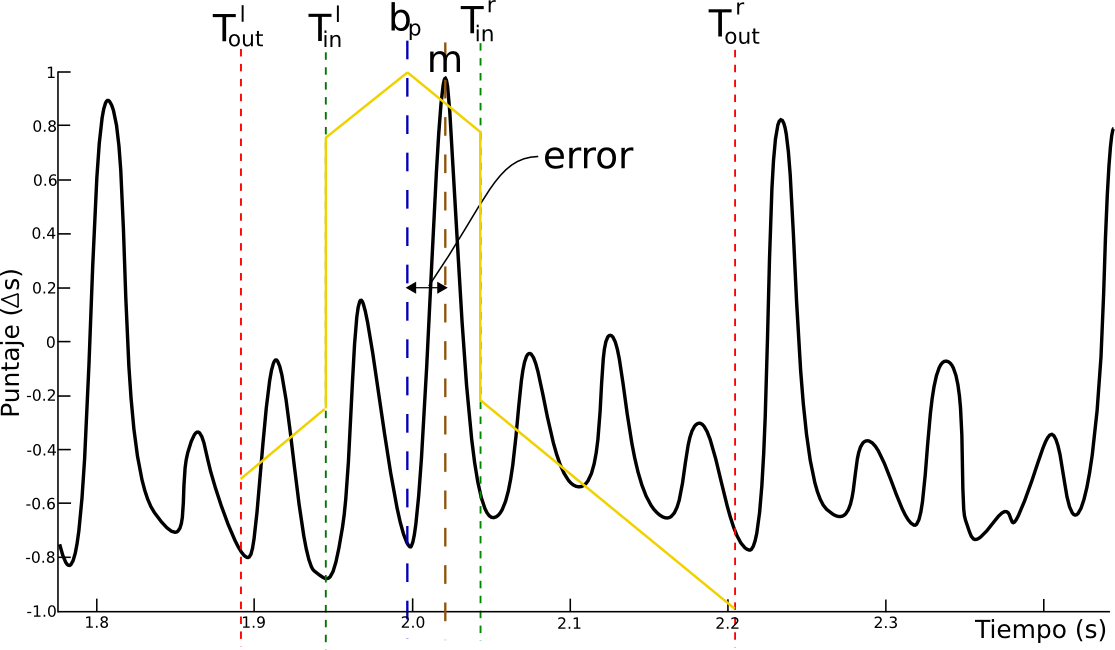
\includegraphics[width=.8\textwidth]{./pics/graficamejor.png}
  \end{center}
  \vspace{-10pt}
  \caption{Niveles de tolerancia}
  \label{fig:grafica}
\end{figure}

En consecuencia aparecen 2 claros escenarios distintos: o bien que el máximo local del Flujo Espectral se encuentre en la región \emph{inner}, o bien que se encuentre en la región \emph{outer}.\\

\begin{itemize} \item Máximo local en región \emph{inner}\end{itemize}
En este caso se considera que el agente está siguiendo los beats de la pieza de buena manera y lo único que se realiza es un ajuste fino de período y fase según sigue:
$$
\begin{cases}
P_i = P_i+0.25\;error\\
\phi_i = \phi_i+0.25\;error
\end{cases}
$$

\begin{itemize} \item Máximo local en región \emph{outer} \end{itemize}
Este caso corresponde a desviaciones mayores que el caso anterior, donde el agente mantiene su período y fase pero para hacer frente a variaciones de tempo repentinas crea 3 ``hijos'' ($C_1$,$C_2$,$C_3$) para seguir 3 alternativas posibles combinando variaciones de \emph{timing} (fase) y \emph{tempo} (período), según sigue:\\
\footnotesize
$$
C_1:
\begin{cases}
P_{C_1}=P_i\\
\phi _{C_1}=\phi _i + error + P_{C_1}
\end{cases}
, \exists m \in T_{out}
$$
$$
C_2:
\begin{cases}
P_{C_2}=P_i+error\\
\phi _{C_2}=\phi _i + error + P_{C_2}
\end{cases}
, \exists m \in T_{out}
$$
$$
C_3:
\begin{cases}
P_{C_3}=P_i+0.5\;error\\
\phi _{C_3}=\phi _i +0.5\;error + P_{C_3}
\end{cases}
, \exists m \in T_{out}
$$

\normalsize

Para que los hijos tengan competitividad respecto al resto de los agentes, se los inicializa con un puntaje igual al 90\% del puntaje del ``padre'' en ese instante.

\subsection{Matado de agentes}

En cualquier punto del análisis, algunas situaciones dan por finalizada la operación de un agente, con los criterios que se explican a continuación:

\begin{itemize}
\item \emph{Replacement}: un agente es matado si llegado al límite de agentes (fijado en 30), es el peor de todos y su puntaje es menor al de otro agente creado más recientemente.
\item \emph{Redundancy}: para mejorar la eficiencia del algoritmo un agente es matado si está duplicando el trabajo de otro con mayor puntaje. Por duplicación de trabajo se entiende que la diferencia entre los períodos no debe ser mayor a $11.6\;ms$ y la diferencia entre las fases no debe superar los $23.2\;ms$.
\item \emph{Obsolence}: un agente es matado si la diferencia entre su puntaje con el mejor agente es mayor al 80\% del mejor puntaje
\item \emph{Loss}: un agente es matado si parece estar ``perdido'', sugerido una cantidad (fijada en 8) de veces consecutivas que la predicción del beat esté por afuera de la región \emph{inner}.
\end{itemize}

\subsection{Agent Referee}

En la versión causal el \emph{referee} va determinando en cada instante cuál es el mejor agente. Mantiene una continua evaluación y le va asignando un puntaje a cada agente respecto a qué tan bueno es el matcheo entre los datos que van llegando y la prediccion del beat. La variación de puntaje en cada instante está dada por la ecuación \ref{ec:ds}.\\

\begin{equation}
\begin{cases}
\Delta s = \left(1-\frac{|error|}{T^r_{out}} \right)\frac{P_i}{P_{max}}SF(m), & \exists m \in T_{in}\\
\Delta s = -\left(\frac{|error|}{T^r_{out}} \right)\frac{P_i}{P_{max}}SF(m), & \exists m \in T_{out}
\end{cases}
\label{ec:ds}\\
\end{equation}
\\
$b_p$ es la predicción del beat, $m$ el máximo correspondiente del Flujo Espectral, y $P_{max}$ el período máximo permitido (correspondiente a $250\;BPM$). El cociente $P_i/P_{max}$ es utilizado para normalizar la función puntaje por el período $P_i$ y es utilizado como una manera de disminuir el puntaje de los agentes más rápidos, que de otra manera tendería a aumentar dado que tienen una mayor cantidad de predicciones de beat. La utilización de un puntaje negativo cuando la predicción cae fuera de la región \emph{inner} infiere una penalización al agente correspondiente.\\

\chapter{Resultados}

\section{Implementación}

En esta sección se presentan algunos detalles en los cuales fue necesario ahondar el estudio para la correcta implementación del algoritmo presentado en la sección \ref{sec:metodologia}, y que resultan interesante destacarlos y documentarlos.\\

%TODO escribir esto bien de aca pa abajo

A la hora de realizar el tracking se planta la posibilidad de pararse en los picos del sF o pararse en las predicciones de beat. centrar la ventana\\


no matar agentes fuera del outer\\

El filtrado de los picos se realiza analizando las distancias entre cada máximo y los mínimos aledaños a él.\\

la matanza de agentes esta pensada para correr en tiempo real. Como nuestro trabajo no lo requería aunque era una buena cosa para conservar, se pueden modificar los criterios de matanza para dejar vivos mas agentes, porque no nos importa que demore un poco mas...\\

Para la versión no causal se puede utilizar un referee elegido al final del proceso de tracking, como se propone en \cite{bib:dixon}, donde se asume que al ir teniendo buenos puntajes a lo largo del tracking, el agente que tenga mayot puntaje al finalizarlo será el mejor agente global.


\section{Señales sintéticas}

Como primer prueba para testear el algoritmo implementado se generan diversas señales sintéticas con período constante. Para ello se convolucionan el sonido de un platillo de batería con un tren de pulsos de frecuencia constante. La prueba siguiente, también sintética consiste en generar una señal con frecuencia variando linealmente a lo largo del tiempo para analizar la performance del algoritmo en el tracking del período variante de una señal.\\

Como primer ejemplo se presenta el caso de una señal de período constante en $90\;BMP$. Los resultados se muestran en las figuras \ref{fig:90BPM}.

\begin{figure} [h!]
\centering
  \subfloat[Autocorrelación del Flujo Espectral]{\label{fig:bpm90autocorr} \centering
  		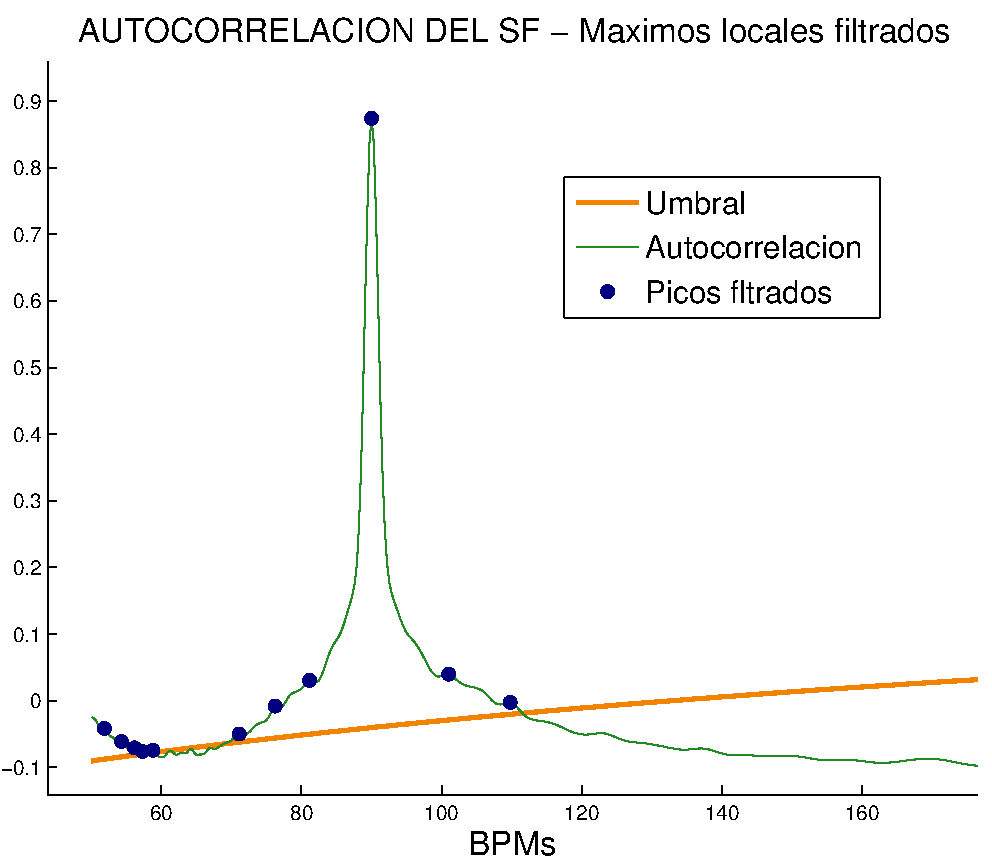
\includegraphics[width=.5\textwidth]{./pics/bpm90autocorr.pdf}} 
  \subfloat[Beats detectados sobre la señal]{\label{fig:bpm90beats} 
  		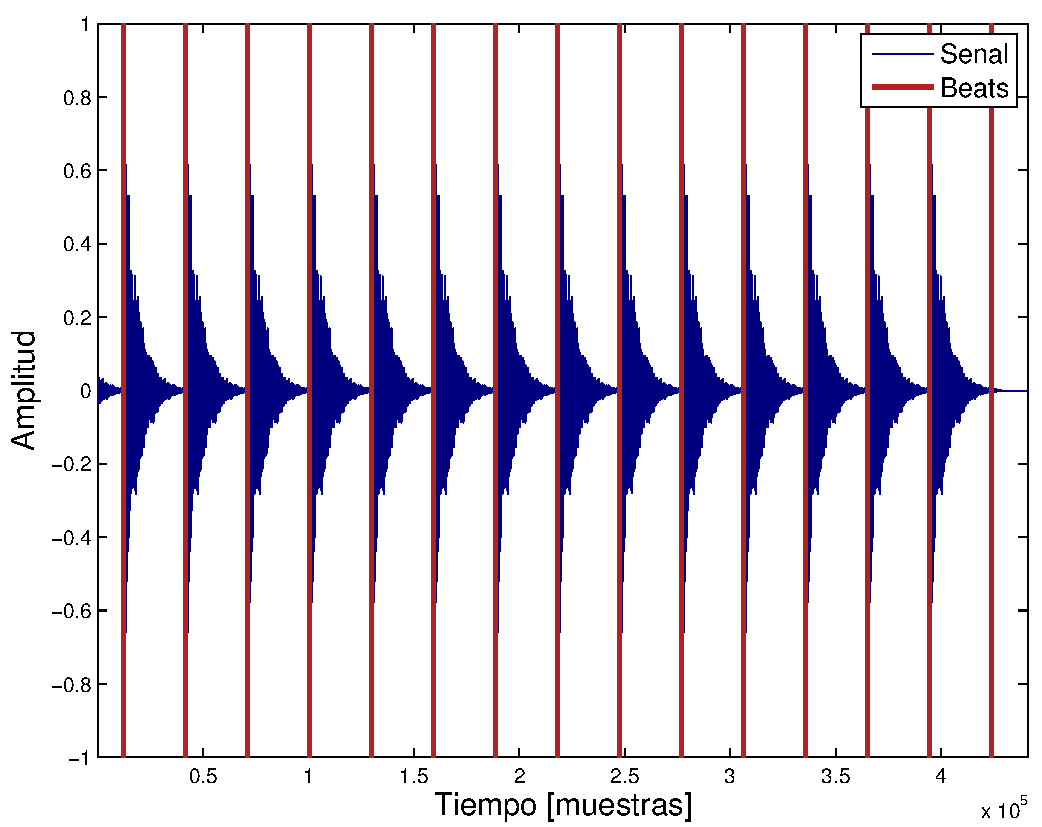
\includegraphics[width=.5\textwidth]{./pics/bpm90beats.pdf}}
  \caption{Señal sintética de 90 BPM}
  \label{fig:90BPM}
\end{figure}

%TODO aca se puede poner los tiempos de los beats y comparar cuantitativamente...

La figura \ref{fig:bpm90autocorr} muestra la autocorrelación del flujo espectral calculado en la \emph{ventana de inducción} mencionada en la sección \ref{sec:pretracking} del Pre-Tracking. Se puede apreciar claramente que el pico marcado que aparece en la figura corresponde con un período de 90BPM, coincidiendo perfectamente con el período de la señal sintética generada. Se puede decir entonces que el Pre-Tracking captó perfectamente el período del beat. Se muestra también el umbral utilizado para filtrar los máximos locales del Flujo Espectral detectados. Por otro lado en la figura \ref{fig:bpm90beats} se muestra una representación de la señal de audio, y sobrepuesta a ella una línea roja en la posición de cada beat detectado. Se puede corroborar el perfecto funcionamiento del algoritmo en este caso.\\

Para analizar la capacidad de adaptación del algoritmo a una pieza musical con tempo variante se genera una señal sintética con período variante entre 90BPM y 100BPM. Los resultados se muestran en la figura \ref{fig:tempovariante}.

\begin{figure} [h!]
\centering
  \subfloat[Beats detectados sobre la señal]{\label{fig:bpm90a100beats} \centering
  		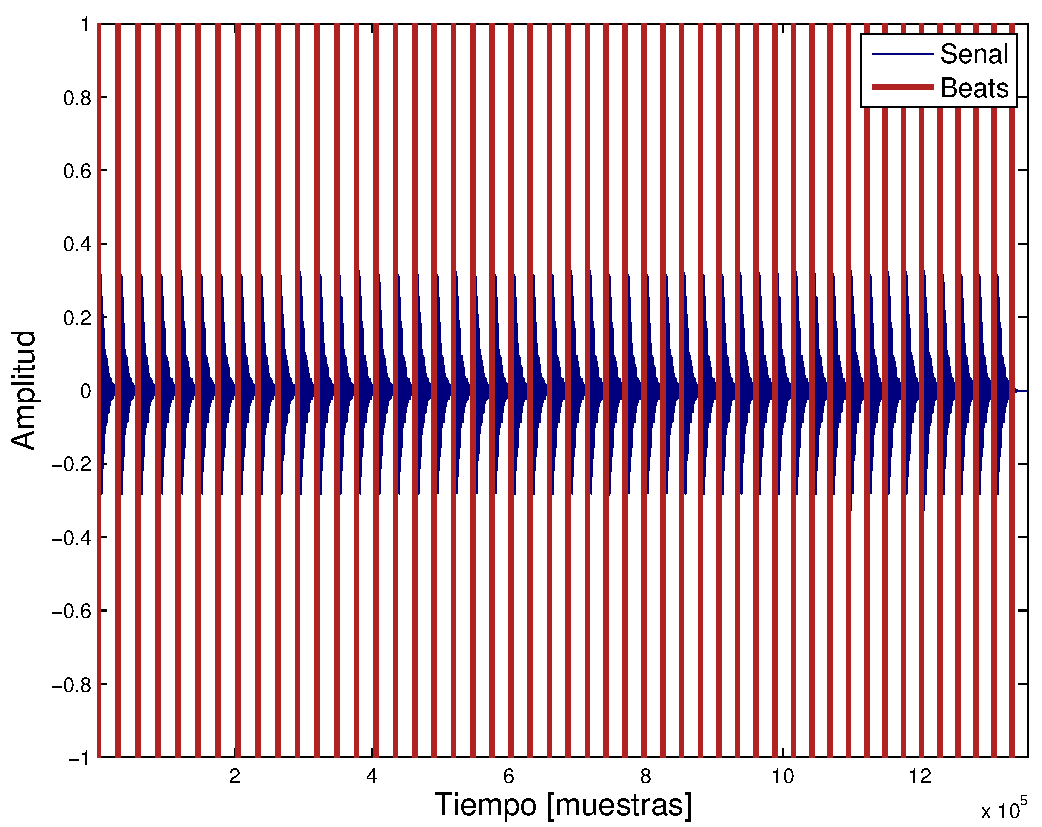
\includegraphics[width=.5\textwidth]{./pics/bpm90a100beats.pdf}} 
  \subfloat[Evolución del tempo]{\label{fig:bpmvariable} 
  		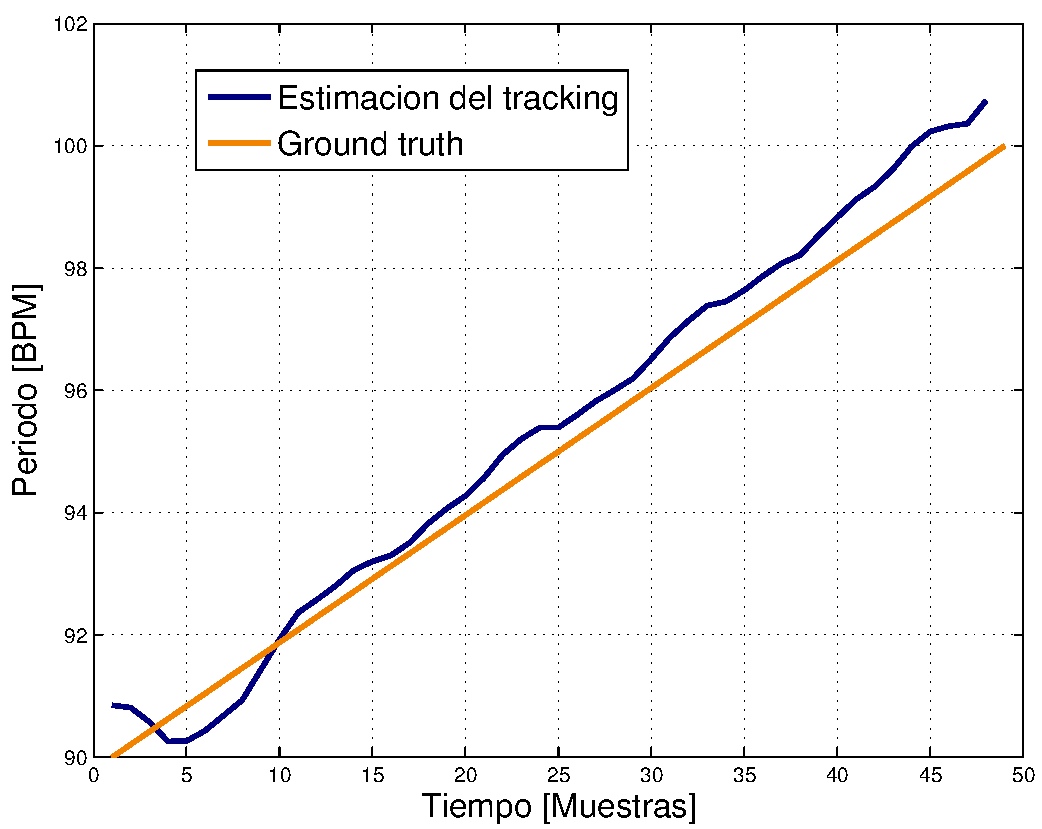
\includegraphics[width=.5\textwidth]{./pics/bpmvariable.pdf}}
  \caption{Señal sintética con tempo variante en forma lineal}
  \label{fig:tempovariante}.
\end{figure}

En la figura \ref{fig:bpm90a100beats} se muestra la señal sintética original con los beats sobrepuestos, donde se puede observar a grandes rasgos que se realiza el tracking en forma exitosa. Por otro lado en la figura \ref{fig:bpmvariable} se puede observar con más detalle la evolución del tempo a lo largo del tiempo. Comparando ambas curvas se puede afirmar que, a menos de un error de alrededor de $0.5\;BPM$, se realiza un tracking exitoso del tempo de la pieza.\\

Una vez realizadas las pruebas sintéticas y corroborado el funcionamiento en situaciones controladas, se procede a testear el algoritmo implementado en situaciones reales, como se pasa a describir en la siguiente sección.

\section{Señales reales}

\subsection{anda bien}

\begin{wrapfigure}{l}{0.45\textwidth}
	\vspace{-25pt}
	\begin{center}
	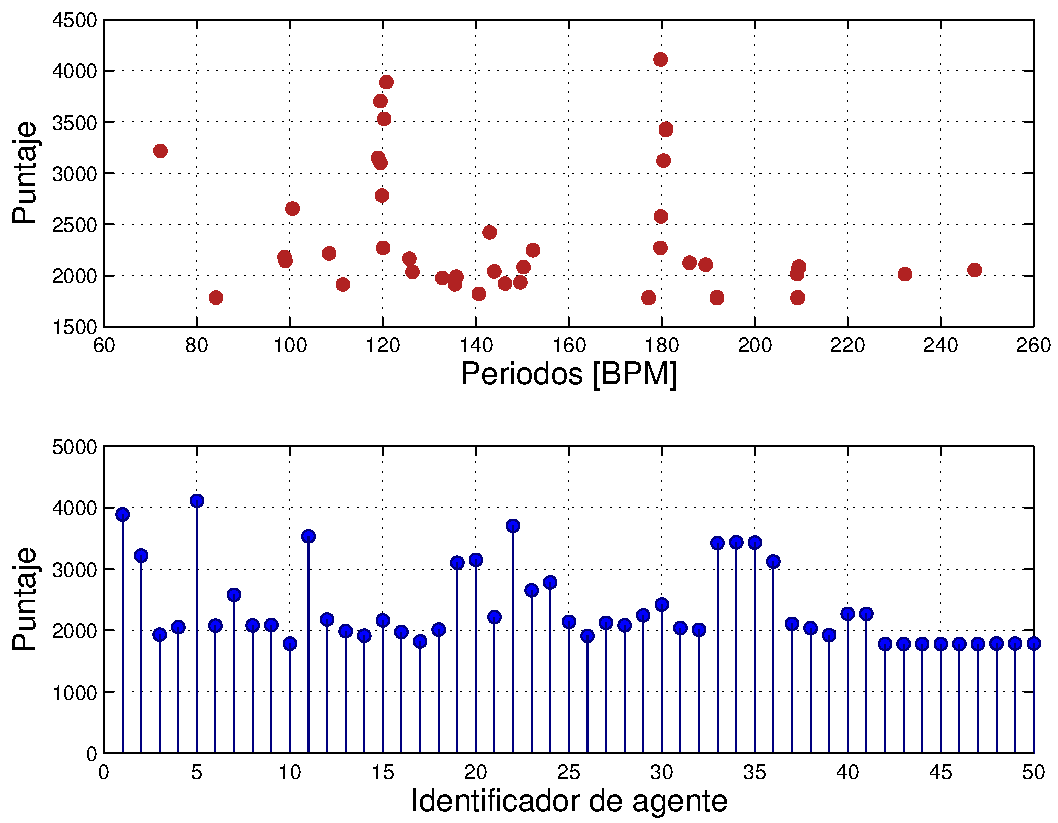
\includegraphics[width=0.4\textwidth]{./pics/train13_agents.pdf}
	\end{center}
	\vspace{-20pt}
	\caption{Agentes finales}
	\label{fig:train13_agents}
	\vspace{-35pt}
\end{wrapfigure}

\begin{figure} [h!]
\centering
  \subfloat[En función de las muestras]{\label{fig:train13_autocorr} \centering
  		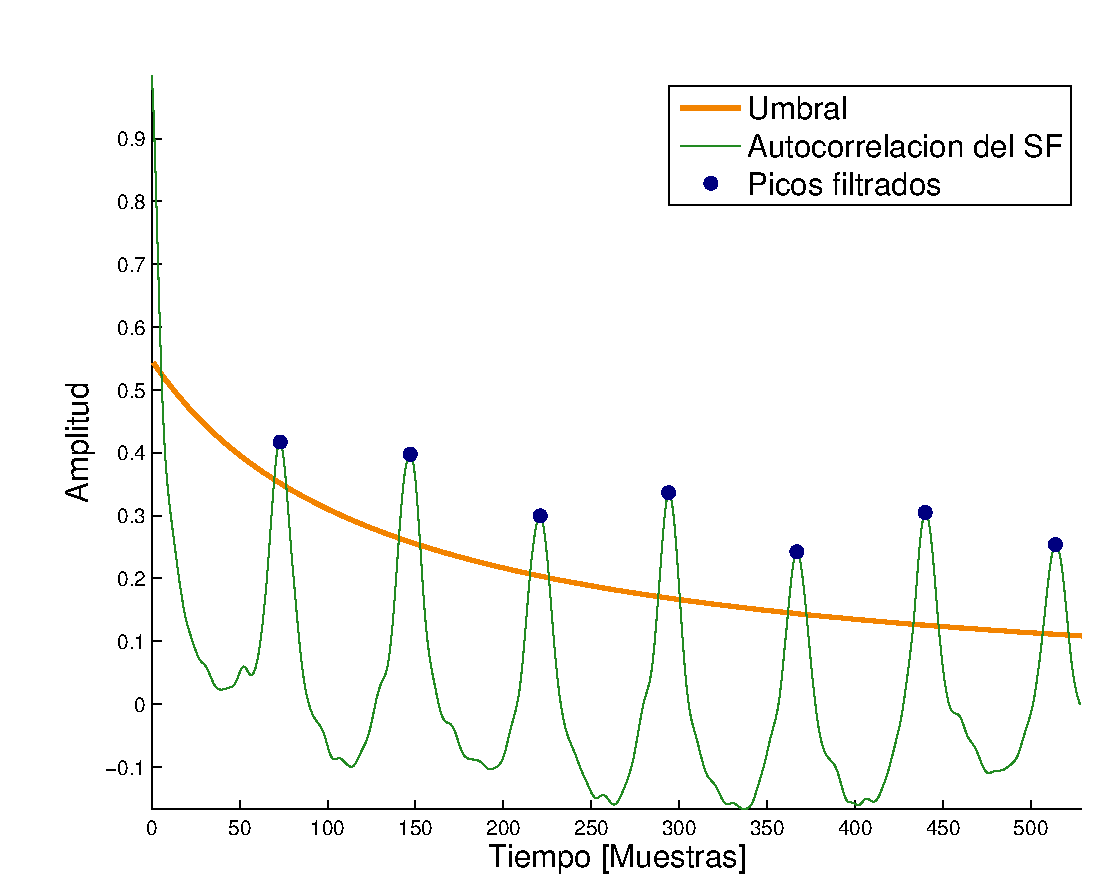
\includegraphics[width=.5\textwidth]{./pics/train13_autocorr.pdf}} 
  \subfloat[Agente número 20]{\label{fig:train13_beats_bien} 
  		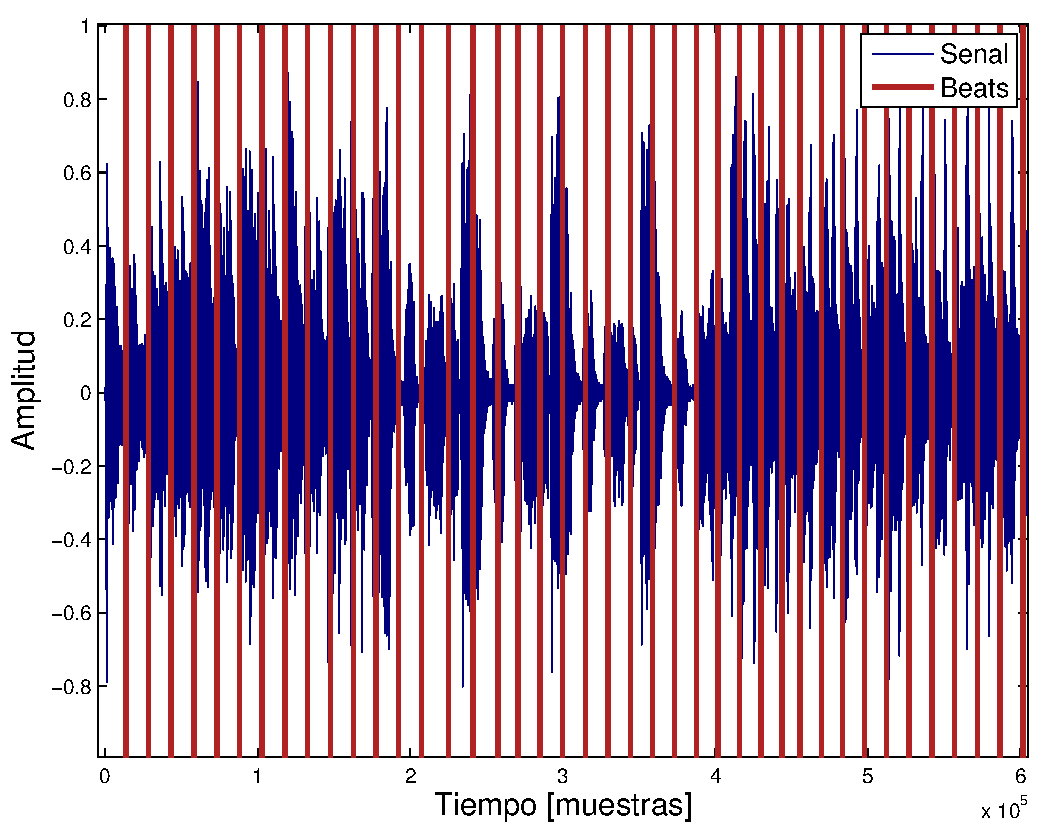
\includegraphics[width=.5\textwidth]{./pics/train13_beats_bien.pdf}}
  \caption{}
  \label{fig:train13}.
\end{figure}



\subsection{anda mal}

\begin{wrapfigure}{l}{0.45\textwidth}
	\vspace{-25pt}
	\begin{center}
	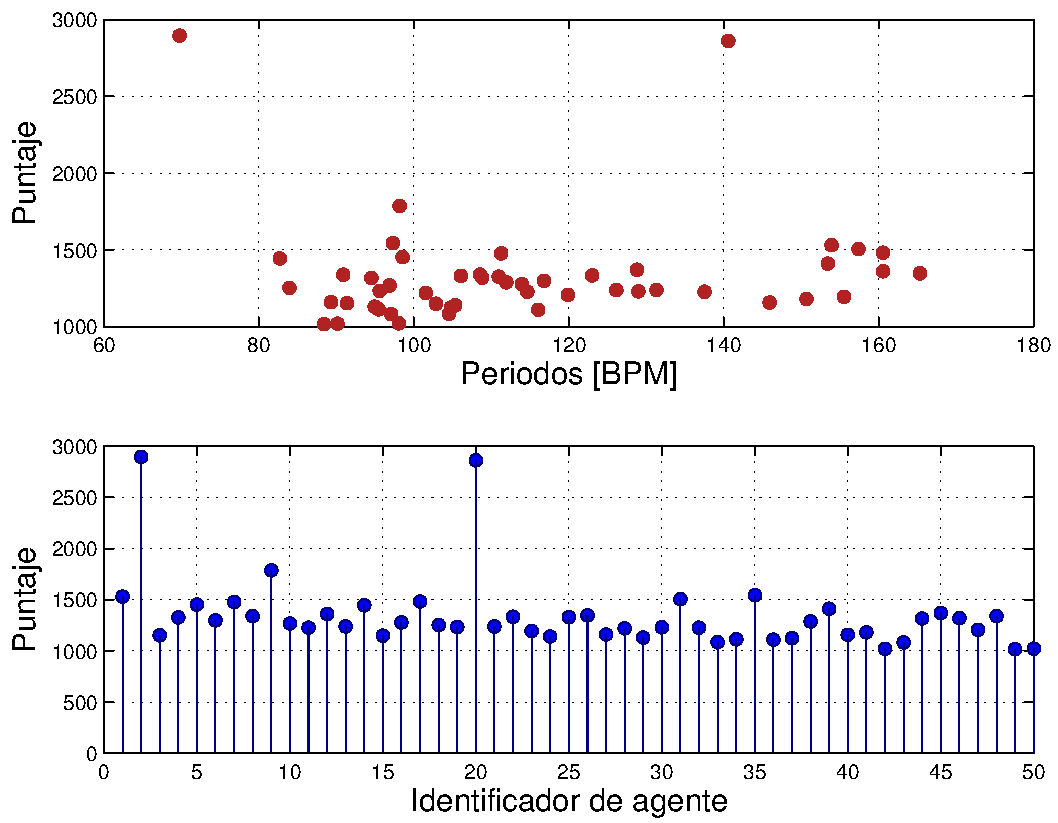
\includegraphics[width=0.4\textwidth]{./pics/train11_agents.pdf}
	\end{center}
	\vspace{-20pt}
	\caption{Agentes finales}
	\label{fig:train11_agents}
	\vspace{-35pt}
\end{wrapfigure}

\begin{figure} [h!]
\centering
  \subfloat[En función de las muestras]{\label{fig:train11_autocorr} \centering
  		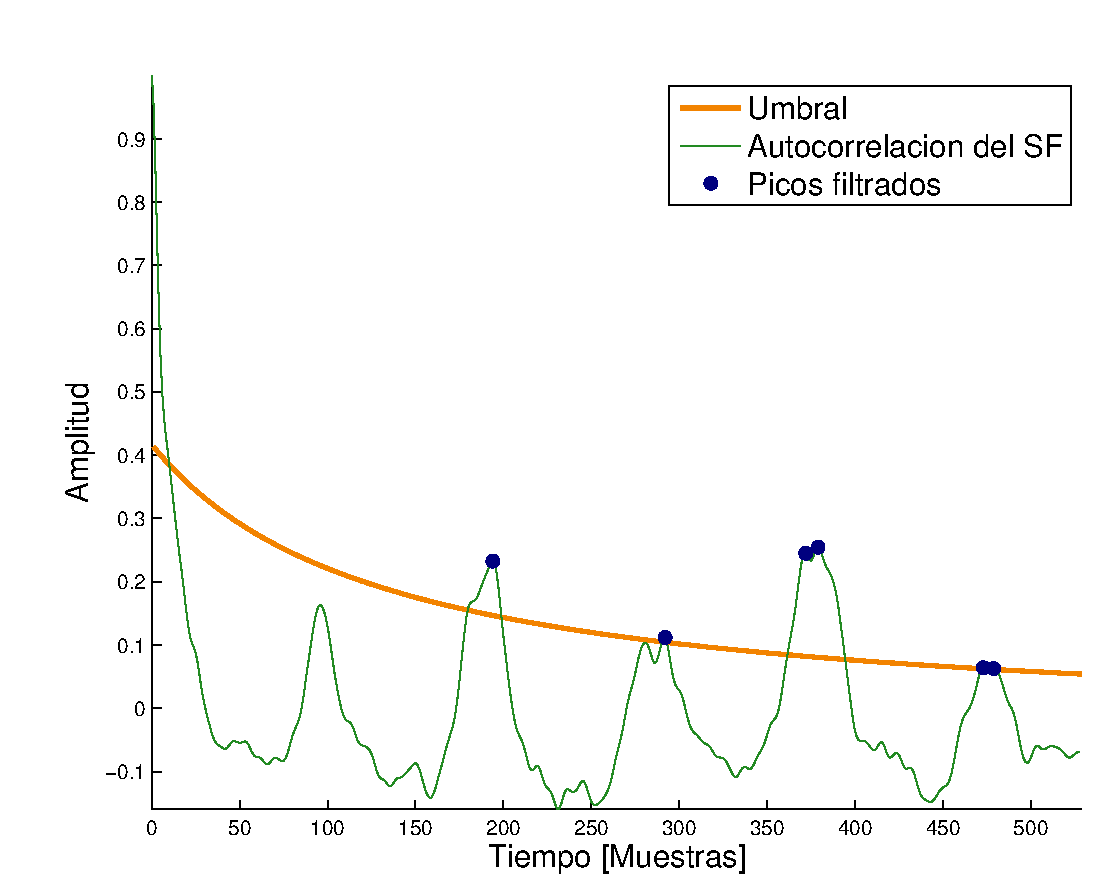
\includegraphics[width=.5\textwidth]{./pics/train11_autocorr.pdf}} 
  \subfloat[En función del período en BPM]{\label{fig:train11_autocorr2} 
  		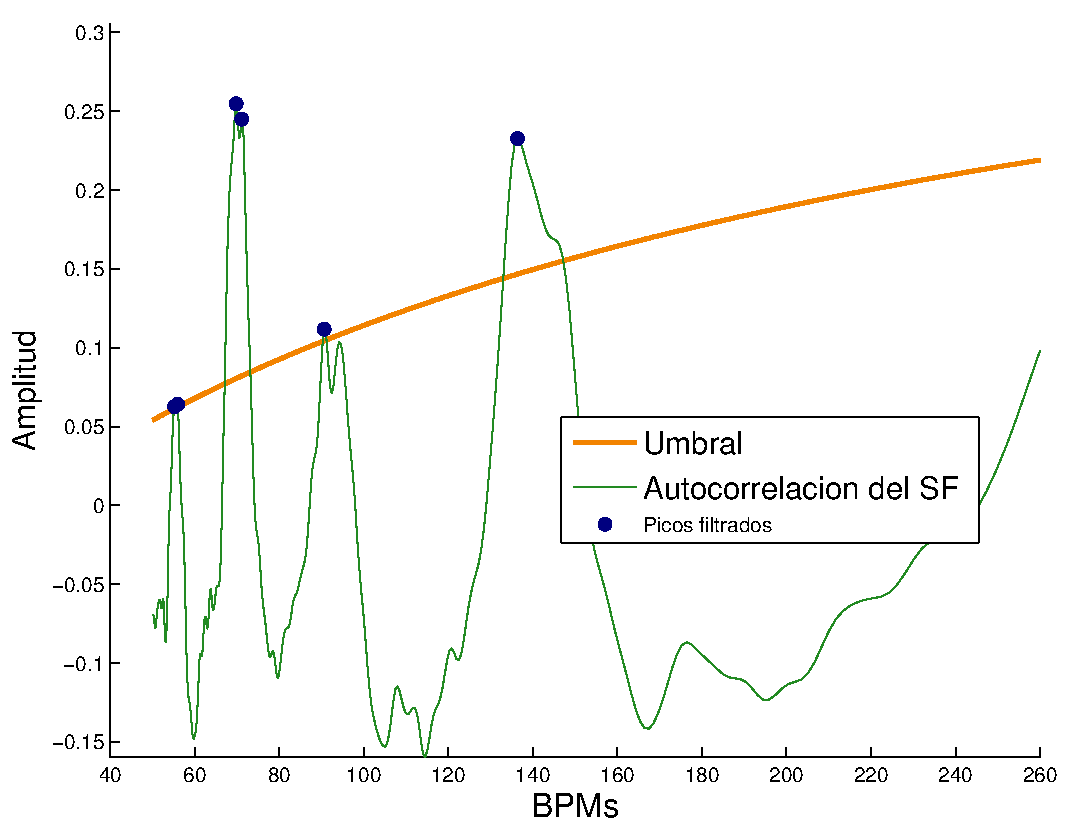
\includegraphics[width=.5\textwidth]{./pics/train11_autocorr2.pdf}}
  \caption{Autocorrelación del Flujo Espectral}
  \label{fig:train11_autocorrelaciones}.
\end{figure}

\begin{figure} [h!]
\centering
  \subfloat[Agente número 2]{\label{fig:train11_beats_lento} \centering
  		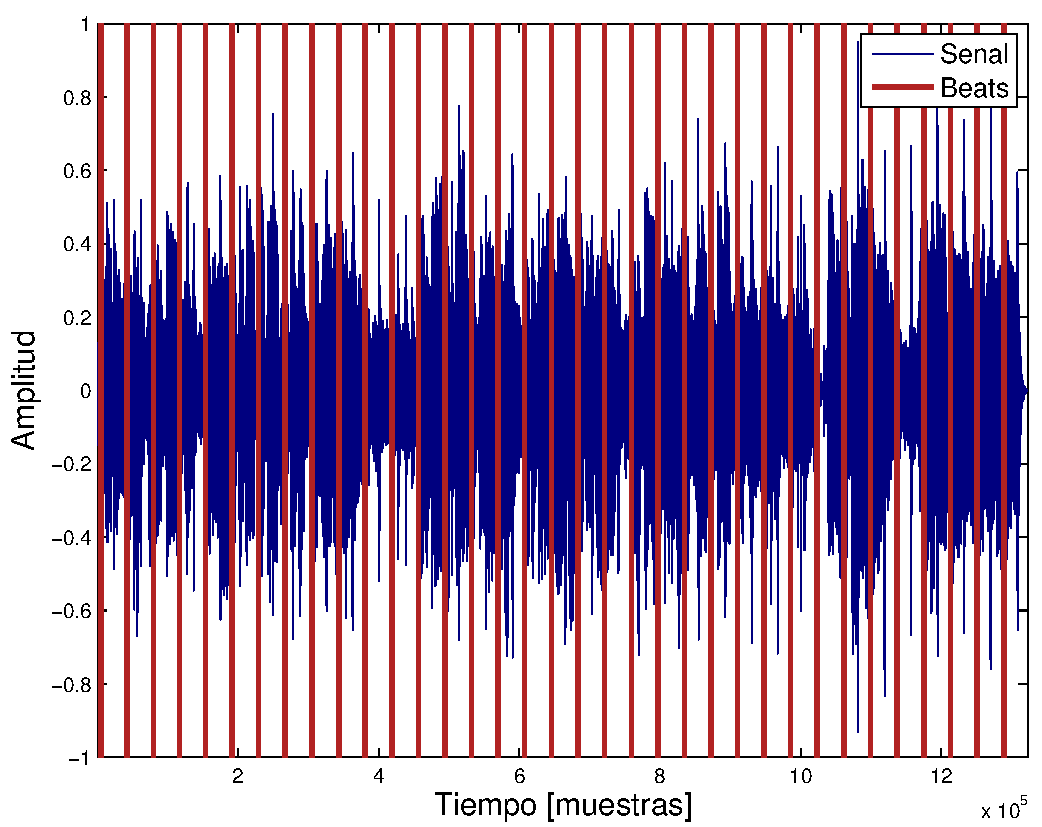
\includegraphics[width=.5\textwidth]{./pics/train11_beats_lento.pdf}} 
  \subfloat[Agente número 20]{\label{fig:train11_beats_bien} 
  		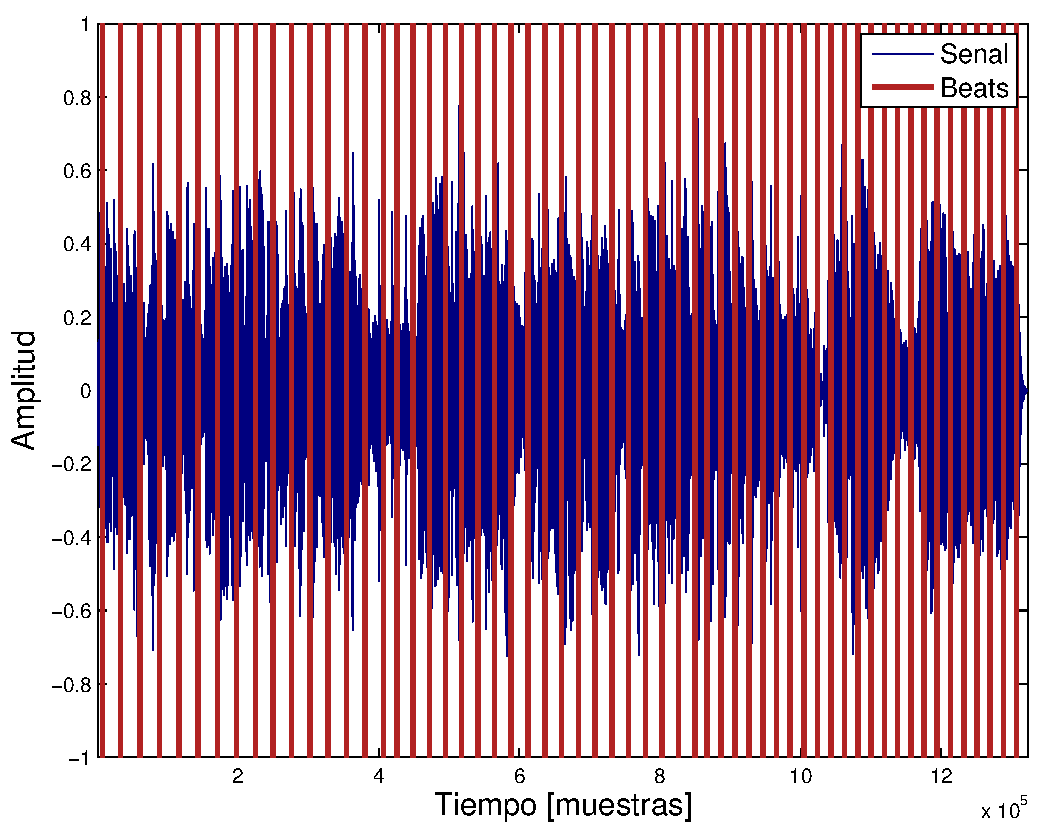
\includegraphics[width=.5\textwidth]{./pics/train11_beats_bien.pdf}}
  \caption{Beats detectados}
  \label{fig:train11_beats}.
\end{figure}


\section{conclusiones}

anda en general muy rico\\

qedaron algunas dudas de implementacion\\

se puede mejorar la parte de la eleccion del agente ganador\\

las debilidades pueden estar en la dificultad de elegir el agente posta... nos pasa a veces q agarramos multiplos...\\

en general esta bastante robusto, no se usan umbrales duros ni cosas demasiado arbitrarias\\

es un sistema muy bien pensado donde se favorece a los mejores y la competencia parece ser un buen camino\\

tiene una buena relación entre la inercia y la rapidez de respuesta\\

en silencios de una cancion sigue marcando el beat como venia por un rato..\\

buenos resultados auditivamente hablando\\


\begin{thebibliography}{99}
\begin{small}

\bibitem{bib:el_posta}Jo\~ao Lobato Oliveira, Fabien Gouyon, Luis Gustavo Martins, Luis Paulo Reis, IBT: A real time tempo and beat tracking system, In \emph{11th International Society for Music Information Retrieval Conference, ISMIR}, 2010.

\bibitem{bib:dixon}S. Dixon. Automatic extraction of tempo and beat from
expressive performances. In \emph{Journal of New Music Research, 30(1):39–58}, 2001.

\bibitem{bib:feature_extraction}S. Dixon. Onset detection revisited. In \emph{in Proceedings of the 9th International Conference on Digital Audio Effects}, pages 133–13, Montreal, Canada, 2006.

\bibitem{bib:y_asi}F. Gouyon, P. Herrera, and P. Cano. Pulse-dependent analyses of percussive music. In \emph{AES 22nd International Conference on Virtual}, Synthetic and Entertainment Audio, 2002.

\end{small}
\end{thebibliography}

\end{document}